\section{Durchführung}
\label{sec:Durchführung}
\subsection{Aufbau}
\begin{figure}[H]
  \centering
  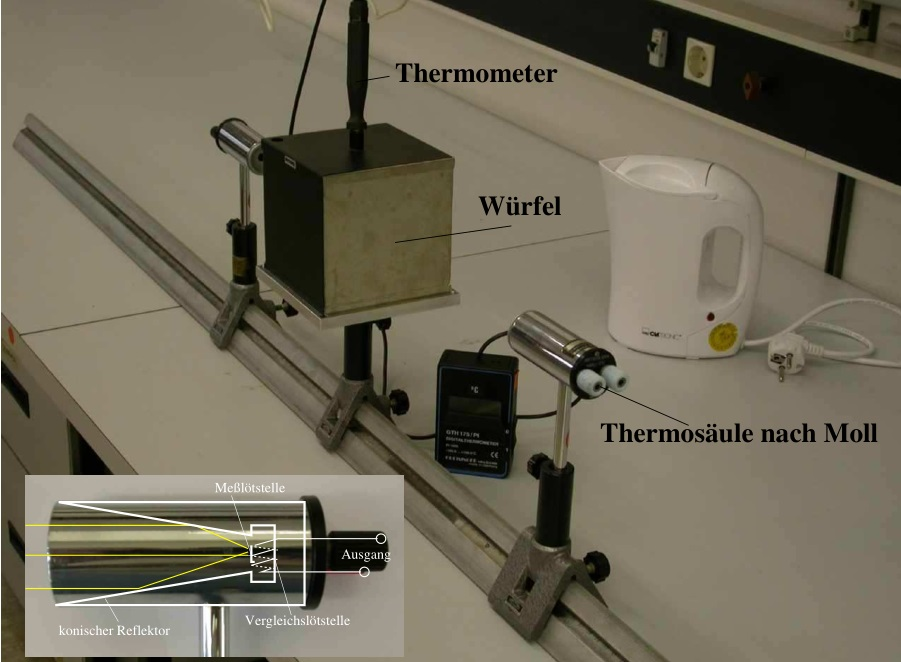
\includegraphics[height=6cm]{Leslie.png}
  \caption{Versuchsaufbau \cite{sample}}
  \label{fig:skizze}
\end{figure}
Um das Stefan-Boltzmann-Gesetz zu überprüfen, besteht der Versuchsaufbau aus einem Lesliewürfel und einer davorstehenden Thermosäule nach Moll.
Der Würfel ist im wesentlichen ein Hohlkörper, dessen vier vertikalen Seitenflächen unterschiedliche farbliche Beschaffenheiten aufweisen.
Die metallischen Oberflächen sind matt, schwarz, glänzend und weiß.
Sie unterscheiden sich demnach in ihrem Emissions- bzw. Absorbtionsvermögen.\\
Um den Würfel von innen zu erwärmen, füllt man ihn mit kochendem Wasser.
Zur Temperaturmessung des Inneren wird ein Thermometer benutzt, welches über ein Loch im Deckel eingeführt wird.
Nach innerer Erwärmung, beginnen die Flächen auf Grund ihrer unterschiedlichen Beschaffenheit verschiedene Wellenlängen an Wärmestrahlung abzugeben.
Zur Messung jener Strahlung wird die Thermosäule benutzt.\\
Sie befindet sich zusammen mit dem Würfel, auf welchen sie gerichtet ist, auf einer Schiene, um einen stabilen Abstand zu gewährleisten.
Die Thermosäule besteht aus einem Zylinder, der kegelförmig ausgehöhlt ist.
Die Wärmestrahlung wird demnach durch die Zylinderöffnung aufgefangen und im Inneren auf eine geschärzte Detektorfläche gebündelt.
In dieser Messlötstelle sitzen in Reihe geschaltete Thermoelemente.
Durch eine Referenzlötstelle, welche die Außentemperatur wahrnimmt, entsteht eine Potentialdifferenz.
Daraus folgt eine messbare Spannung, aus der man die Strahlintensität ableiten kann.\\
Jenes Thermomessgerät ist sehr empfindlich.
Folglich reagiert es auch auf kleinste Störungen der Umgebung, ausgelöst durch beispielsweise die Anwesenheit von Menschengruppen, ob nun stationär oder vorbeigehend.
Sogar die Körperstrahlung der Experimentatoren stellt ein Messrisiko dar.

\subsection{Durchführung}
Zu Messen seien jeweils die Spannungen für alle Flächen des Würfels, einerseits in Abhängigkeit der Temperatur im Inneren des Würfels und andererseits in Abhängigkeit des Abstandes von der Öffnung der Thermosäule zu den Seitenfächen des Würfels. \\
Die Thermosäule wird eingeschaltet.
Zunächst muss jedoch die Offsetspannung $U_{\text{offset},1}$ am Anfang des Experiments ermittelt werden.
Hierzu wird die Spannung notiert, die angezeigt wird, wenn die Thermosäule keine Strahlung aufnimmt.
Zur Abdeckung wird ein schwarzes Stück Pappe verwendet.
Am Ende des Experiments wird erneut der Offset $U_{\text{offset},2}$ ermittelt.
Der Offset muss im Nachhinein linear von den gemessenen Spannungen abgezogen werden.
Zusätzlich wird noch die Raumtemperatur gemessen, da diese ebenfalls bei der Auswertung berücksichtigt werden muss. \\
Nach diesen Vorbereitungen wird der Abstand auf 10cm eingestellt und der Lesliewürfel mit kochendem Wasser befüllt.
Da die Temperatur anfangs sehr schnell abnimmt, beginnt die Messung erst bei 90 Grad.
Von dort an werden immer nach einem bestimmten Temperaturabfall die Spannungen an den vier Seitenfächen gemessen und tabellarisch notiert.
Dieser Vorgang wird solange wiederholt bis der Würfel eine Temperatur von 35 Grad aufweist. \\
Bei einer relativ konstanten Temperatur wird die Abstandsmessung an einer der Flächen durchgeführt.
Diese findet zwischen zwei temperaturabhängigen Messungen statt.
%Diese begann bei 10cm und endete bei 20cm.
Es wird in konstanten Abständen gemessen.
Dabei wird besonders darauf geachtet, dass die Thermosäule beim Verschieben nur am Sockel angefasst wird, um eine möglichst schnelle und genaue Messung zu erzielen.
Danach wird der Abstand wieder auf 10cm zurückgestellt.\\
Nach Abschluss der temperaturabhängigen Messung wird, wie bereits erwähnt, erneut die Offsetspannung ermittelt.
Bei Messabschluss wird die Thermosäule abgeschaltet.
